\subsection{HTTP}
\subsubsection{Network protocols}
Un protocollo è la definizione del comportamento fra due entità che devono comunicare.
\subsubsection{Protocols layer}
Le fuzioni del network sono strutturate con un modello layer, i dati scambiati fra i layer prendo il nome di SDU(Service Data Protocol).
I dati che vengono scambiati fra uno strato protocollare ad un'altro prendo il nome di PDU(Protocol Data Unit).

\subsubsection{TCP(Transmission Control Protocol)}
\begin{itemize}
    \item Trasporto affidabile
    \item controllo del flusso
    \item controllo della congestione
    \item connection-oriented
    \item non fornisce: timing, sicurezza e minimumvthroughput guarantee
\end{itemize}

\subsubsection{UDP(User Datagram Protocol)}
\begin{itemize}
    \item Trasferimento non affidabile
\end{itemize}

\subsubsection{HTTP overview}
Http usa un modello client server, con le seguenti caratteristiche:
\begin{itemize}
    \item user agent: client manda richieste al server(browser, bot, ecc)
    \item origin server: programma che accetta o rifiuta le richieste
    \item local cache: memoria locale(possonoaverla sia il client che il server)
    \item proxy: applicazione intermediaria che svolge il compito sia di client che di server
    \item gateway: applicazione intermediaria(non conosciuta dal client) che permette di nascondere le specifiche del server
\end{itemize}

HTTP usa TCP e sfruttano la porta 80, HTTP non mantiene informazioni riguardo richieste passate del client.
Le connessioni che permette HTTP possono essere persitenti o non, nel caso delle connessioni non persitenti, dopo ogni invio di dati, la connessione viene chiusa.
Nel caso delle connessioni persistenti(Invio di un file grande come un video) la connessione rimane aperta fino all'accertato invio delle risorse.

Per velocizzare l'invio e la ricezione dei pacchetti, si ricorre al pipelining, al posto di inviare un pacchetto ed aspettare la notifica di avvenuta ricezione, con il pipelining si invia i pacchetti in blocchi per ridurre il tempo complessivo.

\subsubsection{Messaggio HTTP}
Il messaggio HTTP è composto di un header e un body, l'header viene popolato da:
\begin{itemize}
    \item caratteristiche di transmissione generali
    \item caratteristiche dell'entità di transmissione
    \item caratteristiche richieste
    \item caratteristiche di risposta
\end{itemize}

Esempio di richiesta HTTP:

\begin{lstlisting}
    GET /index.html HTTP/1.1\r\n
    Host: www-net.cs.umass.edu\r\n
    User-Agent: Firefox/3.6.10\r\n
    Accept: text/html,application/xhtml+xml\r\n
    Accept-Language: en-us,en;q=0.5\r\n
    Accept-Encoding: gzip,deflate\r\n
    Accept-Charset: ISO-8859-1,utf-8;q=0.7\r\n
    Keep-Alive: 115\r\n
    Connection: keep-alive\r\n
    \r\n
\end{lstlisting}

N.B. \textbackslash r\textbackslash n è la combinazione per andare a capo e, se usata senza altro testo, ha lo scopo di seprare le varie parti del pacchetto come request, header e body.


\subsubsection{Metodi HTTP}
\begin{itemize}
    \item GET: trasferisce la risorsa
    \item HEAD: trasferisce solo l'header
    \item POST: effettua un processo risosa-specifico sul payload
    \item PUT: rimpiazza tutte le rappresentazioni di una certa risorsa
    \item DELETE: elimina tutte le rappresentazioni di una certa risorsa
    \item CONNECT: stabilisci la connessioni con il server
    \item OPRIONS: descrivi le opzioni della comunicazione
    \item TRACE: fai un messsage loop-back
\end{itemize}

\subsubsection{Messaggi HTTP idempotenti e sicuri/non sicuri}
\begin{itemize}
    \item idempotente: Metodo che se chiamato una o cento volte fornisce sempre lo stesso risultato
    \item sicuro: metodo che non modifica la risorsa(GET e POST ecc)
\end{itemize}

\subsubsection{Metodi}
\begin{itemize}
    \item GET: \textbf{Sicuro e idempotente}, usato per richiedere una risorsa
    \item POST: \textbf{Non sicuro e nemmeno idempotente}(perche ripetere la stessa azione porta a creare duplicati), usato per creare/aggiornare una risorsa
    \item PUT: \textbf{Idempotente ma non sicuro}, usato per aggiornare o creare una risorsa
    \item DELETE: \textbf{Idempotente ma non sicuro}, elimina le risorse specificate
    \item HEAD: \textbf{Sicuro e idempotente}, usato per richiedere l'header di una risorsa.
    Usato per controllarer la validità di un URL, ecc
\end{itemize}

\subsubsection{Caratteristiche dell'header HTTP}
\begin{itemize}
    \item User-agent: Descrive il client che ha fatto la richiesta
    \item Referer: URL del'elemento dal quale arriva la richiesta URL
    \item Host: Dominio e porta ai quali fare la richiesta
    \item From: utilizza la mail e l'user-agent della persona che fa la richiesta
    \item Range: specifica la grandezza della risorsa(utile nei download)
    \item Accept, Accept-Charset, Accept-Encoding, Accept-Language: formati di negoziazione per permettere al client e al server di usare le stesse Tecnologie.
    \item If-Modified-Since, If,Unmodified-Since: usato nelle richieste HTTP condozionali!!
    \item Authorization, Proxy-Authorization
\end{itemize}

\subsubsection{Codici di stato per HTTP}
\begin{itemize}
    \item 1xx - informazionale
    \item 2xx - successo
    \item 3xx - reindirizzato
    \item 4xx - errore del client
    \item 5xx - errore del server
\end{itemize}

\subsubsection{Cookies}
I Cookies vengono solitamente utilizzati per autenticazione, carrelli della spesa, raccomandazioni e mantenimento dello stato dell pagina web.


\begin{figure}[h!]
	\centering
	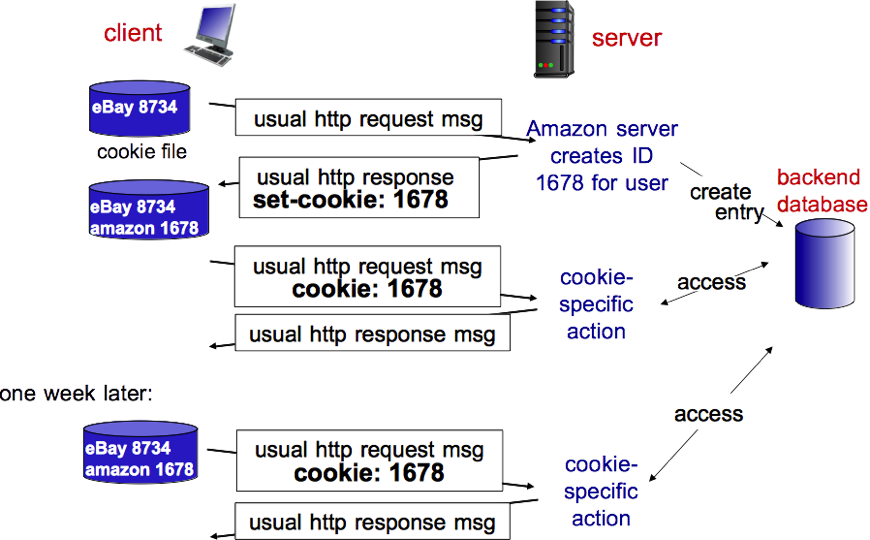
\includegraphics[width=0.6\linewidth]{imgs/1 - cookies.png}
	\caption{Cookies}
	\label{fig:Cookies}
\end{figure}

\subsubsection{Proxy}
Un proxy è un intermediario che ha sia funzioni client che server.
\subsubsection{Web caching}
\begin{figure}[h!]
    \centering
    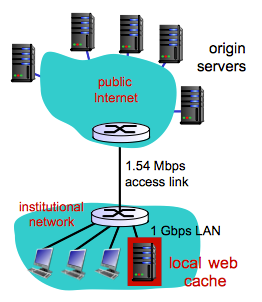
\includegraphics[width=0.3\linewidth]{imgs/2 - web cache.png}
    \caption{Esempio di web caching}
    \label{fig:WebCache}
\end{figure}